\documentclass[12pt]{article}

\usepackage[margin=2.5cm]{geometry}
\usepackage{tikz}
\usepackage{amsmath}
\usepackage{mathtools}
\usepackage{graphicx}
\usepackage{physics}
\usepackage{bm}
\usepackage[colorlinks=true,linkcolor=blue,citecolor=blue,urlcolor=blue]{hyperref}


\setlength{\parindent}{0pt}
\setlength{\parskip}{0.75em}


\title{Chapter 6: Dynamics of System of Particles}
\author{İskender Yalçınkaya, PhD}
\date{\today}

\begin{document}
\maketitle


In the previous chapter, we studied motion under central forces and examined the two-body problem, showing how the motion of two interacting particles can be reduced to an equivalent one-body problem using the center-of-mass and relative coordinates.

We now extend our discussion to systems consisting of an arbitrary number of interacting particles. In such systems, each particle may experience both external forces, originating outside the system, and internal forces, arising from interactions with other particles within the system. Although the motion of individual particles can be complicated, the collective behavior of the system can often be described through a few fundamental quantities.

In this chapter, we develop the general dynamics of systems of particles by studying the center of mass, total linear and angular momentum, and energy. We will examine how internal and external forces affect these quantities and establish the conditions under which the corresponding conservation laws hold.

\section{Center of Mass}

Consider a system consisting of $N$ discrete particles with masses $m_1,m_2,\ldots,m_N$ and position vectors $\vb{r}_1,\vb{r}_2,\ldots,\vb{r}_N$, measured relative to a common origin as shown in Fig.~\ref{fig:center-of-mass}(a). The total mass of the system is
\[
    m_{\text{tot}} = \sum_{i=1}^{N} m_i.
\]
The \emph{center of mass} is defined as the mass-weighted average of the particle positions:
\begin{equation}
    \vb{r}_{\text{cm}} = \frac{1}{m_{\text{tot}}}
    \sum_{i=1}^{N} m_i\vb{r}_i.
    \label{eq:center-of-mass-discrete}
\end{equation}
The center of mass represents the average position of the mass distribution. Its location depends only on the masses and positions of the particles, not on the forces acting on them. The concept of center of mass is particularly useful when studying the overall motion of a system without considering the individual motion of every particle. For example, if all particles move in the same direction with the same velocity, the entire system can be treated,as far as its translational motion is concerned, as a single particle of mass $m_{\text{tot}}$ moving with that velocity. Similarly, although the Earth rotates about its own axis while orbiting the Sun, we can approximately describe its orbital motion by treating the Earth as a point particle located at its center of mass, without considering its rotation. In collisions, the center of mass allows us to separate the overall motion of the system from the relative motion of the colliding bodies, simplifying the analysis of momentum conservation. The center of mass is also important in problems involving balance and stability. For example, an object resting on a horizontal surface under gravity remains stable against tipping as long as the vertical line through its center of mass falls within its base of support.

\begin{figure}[!h]
    \centering
    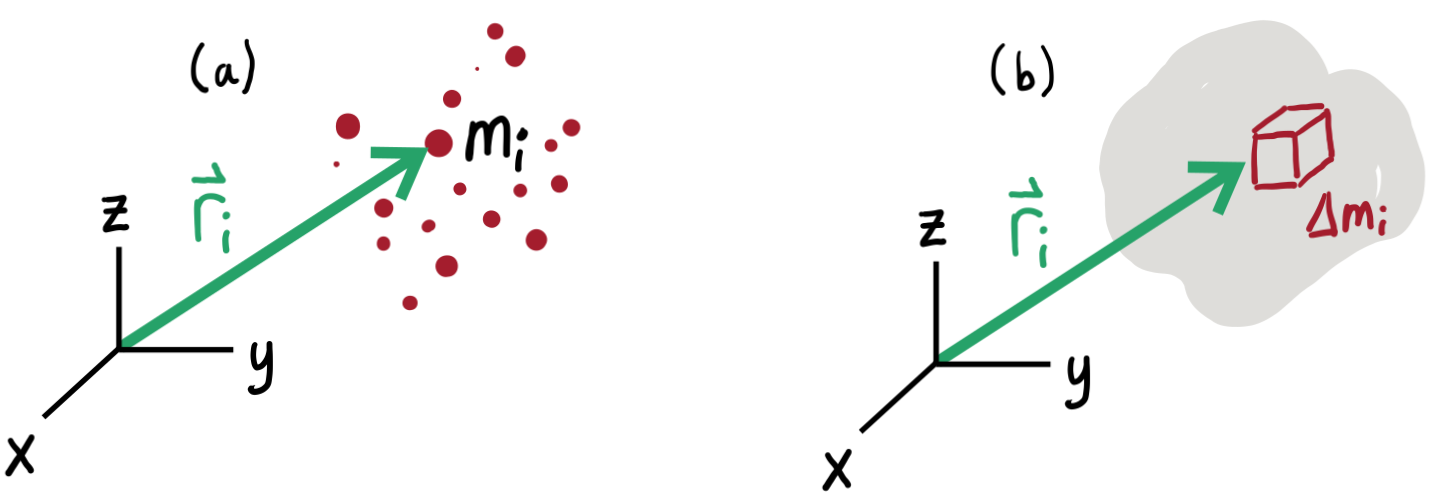
\includegraphics[width=0.8\textwidth]{figures/center-of-mass.png}
    \caption{(a) Discrete distribution of masses. (b) Continuous distribution of masses.}
    \label{fig:center-of-mass}
\end{figure}

If the mass distribution is continuous, we can discretize it into small mass elements as shown in Fig.~\ref{fig:center-of-mass}(b). The center of mass then can be defined as
\[
    \vb{r}_{\text{cm}} = \frac{1}{m_{\text{tot}}}\sum_i \vb{r}_i\Delta{m_i}
\]
where $\Delta{m_i}$ is the mass of the $i$th element. As the size of the mass elements approaches zero, the sum becomes an integral:
\[
    \vb{r}_{\text{cm}} = \lim_{\Delta m \to 0} \frac{1}{m_{\text{tot}}}\sum_i \vb{r}_i\Delta{m_i}=\frac{1}{m_{\text{tot}}}\int \vb{r}\,dm,
\]
where $dm$ is the mass of an infinitesimal element located at position $\vb{r}$. The total mass is given by
\begin{equation}
    m_{\text{tot}} = \int dm.
\end{equation}
In solving problems, it is often convenient to express the mass element in terms of the density functions and a volume element $dV$:
\begin{itemize}
    \item \emph{Linear mass density}: It is defined for one dimensional mass distributions, and it represents the mass per unit length: $dm = \lambda(x)dx$, where $\lambda(x)$ is the linear mass density.
    \item \emph{Surface mass density}: It is defined for two-dimensional mass distributions, and it represents the mass per unit area: $dm = \sigma(x,y)dA$, where $\sigma(x,y)$ is the surface mass density.
    \item \emph{Volume mass density}: It is defined for three-dimensional mass distributions, and it represents the mass per unit volume: $dm = \rho(x,y,z)dV$, where $\rho(x,y,z)$ is the volume mass density.
\end{itemize}
With these definitions, the center of mass for a volume mass distribution in general can be expressed as
\begin{equation}
    \vb{r}_{\text{cm}} = \frac{1}{m_{\text{tot}}}\int \vb{r}\,dm = \frac{1}{m_{\text{tot}}}\int \vb{r}\,\rho(x,y,z)dV.
\end{equation}


\section{Basic Definitions Revisited}

Differentiating the position vector of the center of mass as given in Eq.~\eqref{eq:center-of-mass-discrete} with respect to time once and twice, assuming constant particle masses, gives the velocity and acceleration of the center of mass:
\begin{equation}
    \vb{v}_{\text{cm}} = \dot{\vb{r}}_{\text{cm}}
    = \frac{1}{m_{\text{tot}}}\sum_{i}m_i\vb{v}_i \qquad\text{and}\qquad
    \vb{a}_{\text{cm}} = \ddot{\vb{r}}_{\text{cm}}
    = \frac{1}{m_{\text{tot}}}\sum_{i}m_i\vb{a}_i,
    \label{eq:velocity-acceleration-center-of-mass}
\end{equation}
Here, we only indicate that the summation is over $i$ meaning that is over all particles in the system. Therefore, $\vb{v}_{\text{cm}}$ and $\vb{a}_{\text{cm}}$ are weighted sums of the velocities and accelerations of the individual particles, respectively, like $\vb{r}_{\text{cm}}$ itself. The total linear momentum of the system is the vector sum of the momentum of the individual particles:
\[
    \vb{p}_{\text{tot}} = \sum_{i}m_i\vb{v}_i.
\]
By using $m_{\text{tot}}\vb{v}_{\text{cm}} = \sum_i m_i\vb{v}_i$, we have
\begin{equation}
    \vb{p}_{\text{tot}} = m_{\text{tot}}\vb{v}_{\text{cm}}.
    \label{eq:total-momentum-center-of-mass}
\end{equation}
This result shows that the total linear momentum of a system of particles is equal to the momentum of a single particle having the total mass $m_{\text{tot}}$ and moving with the velocity of the center of mass. Or shortly, the total momentum of a system is the same as the momentum of its center of mass. The angular momentum of a system of particles about a fixed point is the vector sum of angular momenta of the individual particles:
\[
    \vb{L}_{\text{tot}} = \sum_i \vb{L}_i = \sum_{i}\vb{r}_i\times m_i\vb{v}_i.
\]

\section{Motion of the Center of Mass}
From Eq.~\eqref{eq:velocity-acceleration-center-of-mass}, Newton's second law for system of particles can be expressed in terms of the center of mass as
\[
    \vb{a}_{\text{cm}} = \frac{1}{m_{\text{tot}}}\sum_{i}m_i\vb{a}_i = \frac{1}{m_{\text{tot}}}\sum_{i}\vb{F}_i.
\]
where $\vb{F}_i$ is the total force acting on particle $i$. This can be written as
\begin{equation}
    m_{\text{tot}}\vb{a}_{\text{cm}} = \sum_{i}\vb{F}_i.
    \label{eq:motion-center-of-mass}
\end{equation}
Therefore, the total force acting on a system of particles, $\sum_i \vb{F}_i$, accelerates the center of mass of the system. We will write the force acting on the $i$th particle as the sum of the external force $\vb{F}_i^{\mathrm{ext}}$ and the internal forces $\vb{F}_{ij}$ exerted by all other particles $j$ in the system:
\begin{equation}
    \vb{F}_i = \vb{F}_i^{\mathrm{ext}} + \sum_{j}\vb{F}_{ij}, 
    \label{eq:force-on-particle}
\end{equation}
where $\vb{F}_{ij}$ is the force exerted on particle $i$ by particle $j$ and $\vb{F}_i^{\mathrm{ext}}$ is the external force acting on particle $i$. A particle does not exert a force on itself by definitions, and hence $\vb{F}_{ii} = 0$. The reason we separate the forces into external and internal components is to put a boundary between the system and the rest of the universe. In other words, here we implicity defining the notions of a \emph{system} and its \emph{environment} as shown in Fig.~\ref{fig:system-environment}. By this way, we can examine then how the system affects itself and how it is affected by its environment seperately in terms of our previous definitions for motion.
\begin{figure}[!h]
    \centering
    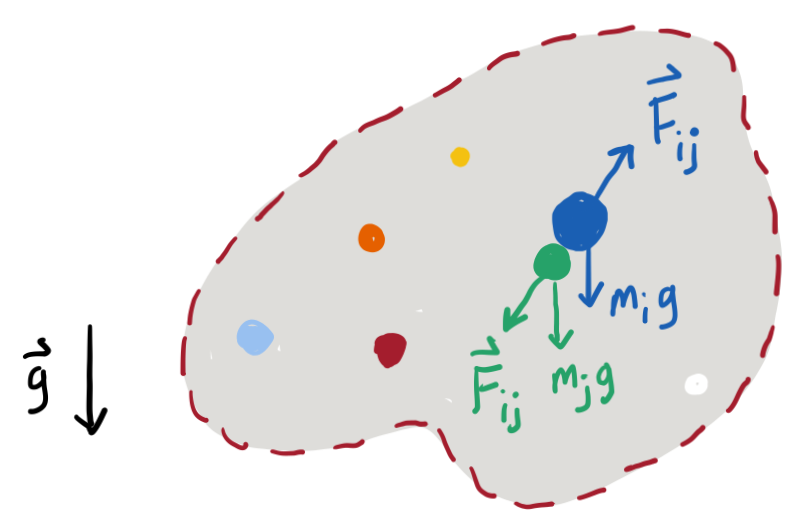
\includegraphics[width=0.5\textwidth]{figures/system-environment.png}
    \caption{A pictorial illustration of a system (gray-shaded area) and its environment (the rest; beyond the dashed line which is the boundary of the system). The system consists of $N$ particles which are bound to live within the system, each of which may experience both external forces (in this case it is gravity) from the environment and internal forces (in this case collisions) from other particles within the system.}
    \label{fig:system-environment}
\end{figure}
By inserting Eq.~\eqref{eq:force-on-particle} into Eq.~\eqref{eq:motion-center-of-mass}, we obtain
\[
    m_{\text{tot}}\vb{a}_{\text{cm}} = \sum_{i}\vb{F}_i^{\mathrm{ext}} + \sum_{ij}\vb{F}_{ij}.
\]
We know that the internal forces satisfy Newton's third law, $\vb{F}_{ij}=-\vb{F}_{ji}$, so that their sum vanishes:
\[
    \sum_{ij}\vb{F}_{ij}=0.
\]
Therefore, the net force acting on the system is simply the sum of the external forces:
\begin{equation}
    m_{\text{tot}}\vb{a}_{\text{cm}} = \sum_{i}\vb{F}_i^{\mathrm{ext}} = \vb{F}_{\mathrm{ext}}.
\end{equation}
Thus, the center of mass moves as if the entire mass
of the system were concentrated at that point and
the net external force acted on it. In particular, if the net external force vanishes, the center of mass moves with constant velocity, or it stays at rest, regardless of the internal motion of the particles. By differentiating the total momentum of the system as given in Eq.~\eqref{eq:total-momentum-center-of-mass} with respect to time, we can also write
\begin{equation}
    \dot{\vb{p}}_{\text{tot}} = m_{\text{tot}}\vb{a}_{\text{cm}} = \vb{F}_{\mathrm{ext}}.
    \label{eq:momentum-center-of-mass}
\end{equation}
Therefore, net external force acting on a system of particles is equal to the time rate of change of the total linear momentum of the system. Total torque acting on an individual particle is the vector sum of the torques associated with the internal and external forces acting on the particle:
\[
    \bm{\tau}_i = \vb{r}_i \times \vb{F}_i = \vb{r}_i \times \vb{F}_i^{\mathrm{ext}} + \sum_{j}\vb{r}_i \times \vb{F}_{ij},
\]
After summing over all particles, the total torque acting on the system is
\[
    \bm{\tau}_{\text{tot}} = \sum_i \bm{\tau}_i = \sum_i \vb{r}_i \times \vb{F}_i^{\mathrm{ext}} + \sum_{ij}\vb{r}_i \times \vb{F}_{ij}.
\]
The term under the double sum can be written as
\[
\vb{r}_i \times \vb{F}_{ij} + \vb{r}_j \times \vb{F}_{ji} = (\vb{r}_i - \vb{r}_j) \times \vb{F}_{ij}.
\]

\section{Conservation Theorems}
We revisit the conservation theorems for linear momentum, angular momentum, and energy in the context of a system of particles and confirm that they hold under the same conditions as for a single particle. 

\subsection{Conservation of Linear Momentum}
If the system of particles is isolated, meaning that the net external force acting on it vanishes, then from Eq.~\eqref{eq:momentum-center-of-mass}, we have
\[
    \dot{\vb{p}}_{\text{tot}} = 0 \implies \vb{p}_{\text{tot}} = \text{constant}.
\]
This implies that if no net external force acts on a system of particle, the center of mass of the system moves with constant velocity, or it remains at rest.  

\section{Worked Examples}
\subsection{Finding the Center of Mass of a System of Particles}
A system of particles consists of three particles with masses $m_1=2\,\mathrm{kg}$, $m_2=3\,\mathrm{kg}$, and $m_3=5\,\mathrm{kg}$ located at positions $\vb{r}_1=(1,0,0)\,\mathrm{m}$, $\vb{r}_2=(0,2,0)\,\mathrm{m}$, and $\vb{r}_3=(0,0,3)\,\mathrm{m}$. Find the center of mass of the system.

\textbf{Solution:}
The total mass of the system is
\begin{equation}
    M = m_1 + m_2 + m_3 = 2 + 3 + 5 = 10\,\mathrm{kg}.
\end{equation}
The center of mass is given by
\begin{equation}
    \vb{R} = \frac{1}{M}\sum_{i=1}^{3} m_i \vb{r}_i
    = \frac{1}{10}\left(2(1,0,0) + 3(0,2,0) + 5(0,0,3)\right).
\end{equation}
Calculating the components, we have
\begin{align}
    \vb{R} &= \frac{1}{10}\left((2,0,0) + (0,6,0) + (0,0,15)\right) \\
    &= \frac{1}{10}(2,6,15) \\
    &= (0.2, 0.6, 1.5)\,\mathrm{m}.
\end{align}
Thus, the center of mass of the system is located at $\vb{R} = (0.2, 0.6, 1.5)\,\mathrm{m}$.
\end{document}
    